\documentclass[a4paper,12pt,oneside,onecolumn,openany,final]{memoir}

% Preamble
%-----------------------------------------------------------------------------------------
\usepackage{thesis_preamble}

\title{Applications of Galois Theory}
\author{Sandesh Thakuri}
% \supervisor{Tulasi Prasad Nepal}

%------------------------------------------------------------------------------------------

\begin{document}

\frontmatter
% --------------------------------------------------------------------------------------------

\begin{center}
  {\LARGE
    {\bfseries {\MakeTextUppercase {\thetitle}}}} \\

  \vspace{1.5cm}

\begin{figure}[h]
	\centering
	\includegraphics[height=5cm,width=5cm]{pictures/tulogo.png}
\end{figure}

\vspace{2cm}

	THESIS SUBMITTED TO\\ THE
	 CENTRAL DEPARTMENT OF MATHEMATICS\\
	INSTITUTE OF SCIENCE AND TECHNOLOGY\\
	TRIBHUVAN UNIVERSITY \\
	KATHMANDU, NEPAL\\

\vspace{1.5cm}

	BY\\
	{\bfseries SANDESH THAKURI}

\vspace{1.5cm}

SUBMITTED FOR THE\\
PARTIAL FULFILLMENT OF THE REQUIREMENT FOR\\
THE MASTER IN SCIENCE/ARTS (M.SC./M.A.)  DEGREE\\
IN MATHEMATICS\\

\vspace{1.5cm}

MARCH, 2024

\end{center}

%\underbrace{}
\thispagestyle{empty}

\clearpage
\addcontentsline{toc}{chapter}{\bfseries STUDENT DECLARATION}
 %\vspace{-1cm}


\begin{center}
  \includegraphics[width=0.15\textwidth]{pictures/tulogo.png}\\[1.5cm]

    {\Large{\bfseries{STUDENT'S DECLARATION}}}\\[.5cm]

  \end{center}


This thesis entitled ``\textbf{\thetitle}", which has been submitted to the Central Department of Mathematics, Institute of Science and Technology (IOST), Tribhuvan University, Nepal for the partial fulfillment of the Master in Science/Arts (M.Sc./M.A.) Degree  in Mathematics, is a genuine work that I carried out under my supervisor {\color{red} Assoc. Prof. Tulasi Prasad Nepal} and that no sources other than those listed in the Bibliography have been used in this work. Moreover, this work has not been published or submitted elsewhere for the requirement of any degree programme.
\\[1.5cm]
-----------------------\\
\theauthor\\
Batch: $2077$ \\
TU Registration Number: 5-2-37-1874-2016\\ \\
Date: March, 2024

\clearpage
\addcontentsline{toc}{chapter}{\bfseries RECOMMENDATION}

\vspace{-1cm}
\begin{center}
	\includegraphics[width=0.15\textwidth]{pictures/tulogo.png}\\[1.5cm]
	{\Large{\bfseries{RECOMMENDATION}}}\\[.5cm]
      \end{center}

This is to recommend that Mr. \textbf{\theauthor} has prepared this thesis entitled ``\textbf{\thetitle}" for the partial fulfillment of the Master in Science/Arts (M.Sc./M.A.) in Mathematics under my supervision. To my knowledge, this work has not been submitted for any other degree.
He has fulfilled all the requirements laid down by the Central Department of Mathematics, Institute of Science and Technology (IOST), Tribhuvan University (TU), Kirtipur for the submission of the thesis for the partial fulfillment of M.Sc./M.A. Degree in Mathematics.\\

\vspace{1.5cm}
\noindent
..............................\\
Mr. Tulasi Prasad Nepal\\
\textbf {Supervisor}\\
%Central Department of Mathematics\\ Tribhuvan University, Kirtipur\\
Associate Professor\\ \\
Date: March, 2024

\clearpage
 \addcontentsline{toc}{chapter}{\bfseries LETTER OF APPROVAL}

 \begin{center}
 	\includegraphics[width=0.15\textwidth]{pictures/tulogo.png}\\[1.5cm]
 {\Large{\bfseries{LETTER OF APPROVAL}}}\\[.5cm]
\end{center}

\noindent
We certify that the Research Evaluation Committee of the Central Department of Mathematics, Tribhuvan University, Kirtipur approved this research work entitled ``\textbf{\thetitle}" carried out by Mr. \textbf{\theauthor} in the scope and generality as a thesis in the partial fulfillment for the requirement of the M.Sc./M.A. degree in Mathematics.
\\[3.5cm]
\begin{minipage}{0.45\textwidth}
                ......................................\\[2mm]
                (\textbf{External Examiner})\\
                Dr. Santosh Ghimire\\
                Pulchowk Campus,\\
                Institute of Engineering,\\
                Tribhuvan University,\\
                Kathmandu, Nepal.\\
		Date: \thedate
\end{minipage} \hspace{3mm}
%
\begin{minipage}{0.55\textwidth}
                ......................................\\
                (\textbf{Supervisor}) \\
		Assoc. Prof. Tulasi Prasad Nepal \\
		Central Department of Mathematics,\\
                Institute of Science \& Technology,\\
                Tribhuvan University,\\
                Kirtipur, Kathmandu, Nepal.\\[0.1cm]
		Date: \thedate

\end{minipage}\\[3cm]

\begin{center}
  ........................................\\
  	(\textbf{Head of Department})\\
        Prof. Dr. Chet Raj Bhatta\\
        Central Department of Mathematics\\
	 Institute of Science \& Technology\\
	 Tribhuvan University, Kathmandu,
	 Kirtipur,Nepal.\\
	Date: \thedate
\end{center}


\maxtocdepth{subsection} % put 3 levels into the ToC
\tableofcontents  %table of contents

\mainmatter
% ---------------------------------------------------------------------------------------------

\addcontentsline{toc}{chapter}{\bfseries {Symbol Conventions Used}}

\hspace{-7mm}
  {\LARGE {\bfseries {Symbol Conventions}}}

  \vspace{7mm}

Through out the thesis following Symbol Convention has been used.\\[4mm]

\begin{itemize}
\item \textbf{K} \hspace{5mm} a field.
\item \textbf{F} \hspace{5mm} an extension field of the field \textbf{K}
\end{itemize}

\section*{Some Standard Symbols}
\begin{enumerate}
\item \(\mathbb{Z}\) \hspace{5mm} set of integers.
\item \(\mathbb{Q}\) \hspace{5mm} set of rationals.
\item \(\mathbb{R}\) \hspace{5mm} set of reals.
\item \(\mathbb{C}\) \hspace{5mm} set of complex numbers.
\item \(\mathbb{Z}_n\) \hspace{5mm} ring of set of integers modulo \(n\).
\item \(\mathbb{Z}_p\) \hspace{5mm} finite prime field.
  \item AES \hspace{5mm} American Encryption Standard.
\end{enumerate}
\clearpage


\part{Galois Theory}
\chapter{Galois Correspondence}
\section{Structure of a Field Extension}
Let \(F=K(u)\) be a field extension of the field \(K\). Then \(F\) is a vector space over \(K\) generated by \(u\).\\
We have \(u^n \in F\) for all \(n \in \mathbb{Z}\) because F is a field. As \(F\) is a vector space over \(K\); \(F\) consists of all linear combinations of \(u^n \)'s, and the quotients of these linear combinations. A such linear combinations is: \(a_nu^n+a_{n-1}u^{n-1}+...+a_1u+a_0\) which is  given by the polynomial \(f(u)\), where \(f(x)=a_nx^n+a_{n-1}x^{n-1}+...+a_1x+a_0\).\\

So the structure of the extension field \(F=K(u)\) is:\\
\(F= \{\frac{f(u)}{g(u)} \;| \; f,g \in K[x],g(u) \neq 0\}\).\\

\begin{theorem}[Existence of an Extension field]
If K is a field and \(f \in K[x]\) is a polynomial of degree \(n\),then there exists a simple extension field \(F=K(u)\) of K such that \(u\in F\) is a root of \(f\).
\end{theorem}

\subsection{Algebraic and Transcendental element}
\begin{theorem}
Let \(F\) be an extension field of a field \(F\).\\
A map \(\phi:K[X] \rightarrow K[u]\) where \(u \in F\) defined by \(\phi (f(x))=f(u)\)\\
i.e, \(\phi (a_0+a_1x+...+a_nx^n)= a_0+a_1u+...+a_nu^n\) is a ring homomorphism.
\end{theorem}

Thus \( K[x]\) and \(K[u]\) are homomorphic.
  \begin{enumerate}
  \item If \(u\) is transcendental over \(K\) then \(K[u]\) is not a field and \(K[x] \cong K[u]\).
  \item If \(u\) is algebraic over \(K\) then, \(K[x] \ncong K[u]\) because \(Ker\phi\) is non trival and we have,
    \begin{enumerate}
    \item[i)] \(K(u) \cong K[u]\);
    \item[ii)] \(K(u) \cong K[x]/(f)\), where \(f \in K[x]\) is an 'irreducible monic polynomial of degree \(n \geq 1\);
    \item[iii)] \([K(u):K]=n\) and \(\{1_k,u,u^2,...,u^{n-1}\}\) is a basis of the vector space \(K(u) over K\).
    \end{enumerate}
  \end{enumerate}

\begin{theorem}[Isomorphism of Extension fields]
 Let K be a field.\\
 Then 'u' and 'v' are  roots of the same irreducible polynomial \(f \in K[x]\) if and only if there is an isomorphism of fields \(K[u] \cong K[v]\) which sends u onto v and is the identity on \(K\).
\end{theorem}

\section{Galois Group}
Let \(F\) be a field. The set \(AutF\) of all field-automorphisms \(F \rightarrow F \) forms a group under the function composition.\\ \\
Let \(E\) and \(F\) be the extension fields of a field \(K\).\\
If a non-zero field-homomorphism \(\sigma : E \rightarrow F\) is a K-module homomorphism then\\
\(\sigma(k)=\sigma(k1_E)=k\sigma(1_E)=k1_F=k\).\hspace{7mm}
i.e, \(\sigma\) fixes \(K\) element-wise.\\
Conversely, if a field homomorphism \(\sigma : E \rightarrow F\) fixes K element-wise, then \(\sigma\) is a non-zero and for any \(u \in E\), we have, \(\sigma(ku)=\sigma(k)\sigma(u)=k\sigma(u)\)
i.e \(\sigma\) is a K-module homomorphism.\\
\begin{definition}
  A field-automorphism \(\sigma \in Aut F\) which is also K-homomorphism is called K-automorphism. In other words, a field-automorphism \(\sigma \in Aut F\) that fixes K element-wise is called K-automorphism.
\end{definition}

\begin{definition}
  The group of all K-automorphisms of \(F\) is called the Galois group of \(F\) over \(K\) and it is denoted by \(Aut_K^F\).
\end{definition}

\section{Galois extension}
Let \(E\) be an intermediate field and \(H\) be a subgroup of \(Aut_K^F\), then:
\begin{enumerate}
\item[i)] \(H' = \{v \in F \; | \: \sigma(v)=v,\) for all \(\sigma \in H \}\) is an intermediate field of the extension field \(F\) of \(K\);
\item[ii)] \(E' = \{\sigma \in Aut_K^F \; | \; \sigma(u)=u,\) for all \(u \in E\}=Aut_E^F\) is a subgroup of \(Aut_K^F\).
\end{enumerate}

The field \(H'\) is called the fixed field of the subgroup H in F.

\subsection{Fixed Field}
We have,\\
\(H' \rightarrow\) fixed field and \(E' \rightarrow\) \(Aut_E^F\).\hspace{5mm} Let \(Aut_K^F = G\) then the field fixed by it is \(G'\). It is not necessary that the field fixed by \(G\) is \(K\) i.e, \(G'=K\).
\begin{example}
For \(f(x)=x^3-2 \in Q[x]\). Let \(u \in F\) such that \(f(u)=0\) and let \(F=Q[u]\).Then
\(G=Aut_Q^{Q(u)}={1}\) so, \hspace{5mm}\(G'=F \neq K\).\\
\end{example}

\begin{definition}
  Let \(F\) be an extension field of \(K\) such that the fixed field of the Galois group \(Aut_K^F\) is \(K\) itself. Then \(F\) is said to be a Galois extension of \(K\) or Galois over \( K\).
\end{definition}

\section{Fundamental Theorem of Galois Theory}
\begin{theorem}
If \(F\) is a finite dimensional Galois extension of \(K\), then there is a one-to-one correspondence between the set of all intermediate fields of \(F\) over \(K\) and the set of subgroups of the Galois group \(Aut_K^F\) such that:
\begin{enumerate}
\item[i)] the relative dimension of two intermediate fields is equal to the relative index of the corresponding subgroups. In particular \(Aut_K^F\) has order \([F:K]\);
  \item[ii)] \(F\) is Galois over every intermediate field \(E\), but \(E\) is Galois over \(K\) if and only if the corresponding subgroup \(E'= Aut_E^F\) is normal in \(G=Aut_K^F\).In this case \(G/E'\) is isomorphic to the Galois group \(Aut_K^E\) of \(E\) over \(K\).
  \end{enumerate}
\end{theorem}
We already have a correspondence between the intermediate fields and the subgroup of Galois group.\\
That is to each intermediate field \(E\), there is a subgroup \(Aut_E^F\) and to each subgroup \(H\) there is a fixed field \(H'\). But this correspondence is one-to-one if and only if for each intermediate field \(E\), it satisfies \(E''=E\) and for each subgroup \(H\), it satisfies \(H''=H\).

  \subsection{Closed Field and Subgroup}
  We have,
  \begin{enumerate}
  \item[i)] \(F'=1\) and \(K'=G\);
  \item[ii)] \(1'=F\);
    \end{enumerate}

    If \(F\) is Galois over \(K\) then by definition, \(G'=K\). Since \(K'=G\) we have \(K=K''\) if and only if \(F\) is Galois over \(K\).\\

\begin{definition}
  Let \(X\) be an intermediate field or subgroup of the Galois group. \(X\) will be called \textbf{closed} provided \(X=X''\).\\
\end{definition}

\begin{lemma}. If \(F\) is an extension field of \(K\), then there is one-to-one correspondence between the closed intermediate fields of the extension and the closed subgroups of the Galois group, given by \(E \rightarrow E' =  Aut_E^F\).\\
\end{lemma}

\begin{lemma}. Let \(F\) be an extension field of \(K\), \(L\) and \(M\) intermediate fields with \(L \subset M\), and \(H\), \(J\) subgroups of Galois group \(Aut_K^F\) with \(H<J\).
    \begin{enumerate}
    \item[i)] If \(L\) is closed and \([M:L]\) finite, then \(M\) is closed and \([L':M']=[M:L]\);
    \item[ii)] if \(H\) is closed and \([J:H]\) finite, then \(J\) is closed and \([H':J']=[J:H]\);
      \item[iii)] if \(F\) is a finite dimensional Galois extension of \(K\), then all intermediate fields and all subgroups of the Galois group are closed and \(Aut_K^F\) has order \([F:K]\).
\end{enumerate}
\end{lemma}


\subsection{Stable Intermediate}
\begin{lemma}
Let \(F\) be an extension field of K.
      \begin{enumerate}
      \item[i)] If E is a stable intermediate field of the extension, then \(E'=Aut_E^F\) is a normal subgroup of the Galois group \(Aut_K^F\);
        \item[ii)] if \(H\) is a normal subgroup of \(Aut_K^F\), then the fixed field \(H'\) of \(H\) is a stable intermediate field of the extension.
        \end{enumerate}
        \end{lemma}

        \subsection{Proof of the Fundamental Theorem}
        \begin{proof}
From the above section there is one-to-one correspondence between closed intermediate fields of the extension and closed subgroups of the Galois group. But in this case all intermediate fields and all subgroups are closed. Thus follows statement(i) of the theorem.\\

        \(F\) is Galois over \(E\) since \(E\) is closed. \(E\) is finite dimensional over \(K\) since \(F\) is and hence algebraic over \(K\). Consequently, if \(E\) is Galois over \(K\), then \(E\) is stable.
        \(E'=Aut_E^F\) is normal in \(Aut_K^F\). Conversely if \(E'\) is normal in \(Aut_K^F\), then \(E''\) is stable intermediate field. But \(E=E''\) since all intermediate fields are closed and hence \(E\) is Galois over \(K\).\\

       Suppose \(E\) is an intermediate field that is Galois over \(K\). Since \(E\) and \(E'\) are closed and \(G'=K\)(F is Galois over K), we have \(|G/E'|=[G:E']=[E''=G']=[E:K]\). So, \(G/E'=Aut_K^F/Aut_E^F\) is isomorphic to a subgroup of \(Aut_K^F\). But by first part of the theorem, \(|Aut_K^E|=[E:F]\)(since E is Galois over K). This implies \(G/E'=Aut_K^E\).
        \end{proof}


%%% Local Variables:
%%% mode: latex
%%% TeX-master: "n"
%%% End:


%\chapter{Galois Theory}
%\section{Galois Group}
Let \(F\) be a field. ``The set \(AutF\) of all field-automorphisms \(F \rightarrow F \) forms a group under the function composition'' \cite{hunger}.\\[3mm]
\noindent
Let \(E\) and \(F\) be the extension fields of a field \(K\).\\
If a non-zero field-homomorphism \(\sigma : E \rightarrow F\) is a K-module homomorphism then\\
\(\sigma(k)=\sigma(k1_E)=k\sigma(1_E)=k1_F=k\).\hspace{7mm}
i.e, \(\sigma\) fixes \(K\) element-wise.\\
Conversely, if a field homomorphism \(\sigma : E \rightarrow F\) fixes K element-wise, then \(\sigma\) is a non-zero and for any \(u \in E\), we have, \(\sigma(ku)=\sigma(k)\sigma(u)=k\sigma(u)\)
i.e \(\sigma\) is a K-module homomorphism \cite{hunger}.
\begin{definition} \cite{hunger}
  A field-automorphism \(\sigma \in Aut F\) which is also K-homomorphism is called K-automorphism. In other words, a field-automorphism \(\sigma \in Aut F\) that fixes K element-wise is called K-automorphism.
\end{definition}

\begin{definition} \cite{hunger}
  ``The group of all K-automorphisms of \(F\) is called the Galois group of \(F\) over \(K\) and it is denoted by \(Aut_K^F\).''
\end{definition}

\section{Galois extension}
Let \(E\) be an intermediate field and \(H\) be a subgroup of \(Aut_K^F\), then:
\begin{enumerate}
\item[i)] ``\(H' = \{v \in F \; | \: \sigma(v)=v,\) for all \(\sigma \in H \}\)'' \cite{hunger} is an intermediate field of the extension field \(F\) of \(K\);
\item[ii)] ``\(E' = \{\sigma \in Aut_K^F \; | \; \sigma(u)=u,\) for all \(u \in E\}=Aut_E^F\)'' \cite{hunger} is a subgroup of \(Aut_K^F\).
\end{enumerate}

The field \(H'\) is called the fixed field of the subgroup H in F \cite{hunger}.

\subsection{Fixed Field}
We have,\\
\(H' \rightarrow\) fixed field and \(E' \rightarrow\) \(Aut_E^F\).\hspace{5mm} Let \(Aut_K^F = G\) then the field fixed by it is \(G'\). It is not necessary that the field fixed by \(G\) is \(K\) i.e, \(G'=K\).
\vspace{3mm}
\begin{example}
  For \(f(x)=x^3-2 \in Q[x]\). Let \(u \in F\) such that \(f(u)=0\) and let \(F=Q[u]\).Then
  \(G=Aut_Q^{Q(u)}={1}\) so, \hspace{5mm}\(G'=F \neq K\).
\end{example}

\vspace{3mm}
\begin{definition} \cite{hunger}
``Let \(F\) be an extension field of \(K\) such that the fixed field of the Galois group \(Aut_k^F\) is \(K\) itself. Then \(F\) is said to be a Galois extension of \(K\) or Galois over K.''
\end{definition}

\section{Fundamental Theorem of Galois Theory}
\begin{tcolorbox}
\begin{theorem} \cite{hunger}
  ``If \(F\) is a finite dimensional Galois extension of \(K\), then there is a one-to-one correspondence between the set of all intermediate fields of \(F\) over \(K\) and the set of subgroups of the Galois group \(Aut_K^F\) such that:
  \begin{enumerate}
  \item[i)] the relative dimension of two intermediate fields is equal to the relative index of the corresponding subgroups. In particular \(Aut_K^F\) has order \([F:K]\);
  \item[ii)] \(F\) is Galois over every intermediate field \(E\), but \(E\) is Galois over \(K\) if and only if the corresponding subgroup \(E'= Aut_E^F\) is normal in \(G=Aut_K^F\).In this case \(G/E'\) is isomorphic to the Galois group \(Aut_K^E\) of \(E\) over \(K\).''
  \end{enumerate}
\end{theorem}
\end{tcolorbox}

\vspace{2mm}
We already have a correspondence between the intermediate fields and the subgroup of Galois group.\\
That is to each intermediate field \(E\), there is a subgroup \(Aut_E^F\) and to each subgroup \(H\) there is a fixed field \(H'\). But this correspondence is one-to-one if and only if for each intermediate field \(E\), it satisfies \(E''=E\) and for each subgroup \(H\), it satisfies \(H''=H\).

\subsection{Closed Field and Subgroup}
\begin{definition} \cite{hunger}
  ``Let \(X\) be an intermediate field or subgroup of the Galois group. \(X\) will be called \textbf{closed} provided \(X=X''\).''
\end{definition}
\clearpage

\begin{lemma} \cite{hunger}
\begin{enumerate}
\item[i)] If \(F\) is an extension field of \(K\), then there is one-to-one correspondence between the closed intermediate fields of the extension and the closed subgroups of the Galois group, given by \(E \rightarrow E' =  Aut_E^F\).
\item[ii)] If \(F\) is a finite dimensional Galois extension of \(K\), then all intermediate fields and all subgroups of the Galois group are closed and \(Aut_K^F\) has order \([F:K]\).
  \end{enumerate}
\end{lemma}
\vspace{3mm}

\subsection{Stable Intermediate}
\begin{definition} \cite{hunger}
  An intermediate field \(E\) of \(F\) over \(K\) is said to be stable intermediate if \(\sigma(E) \subseteq E\) for every \(\sigma \in Aut_K^F\) .
\end{definition}

\begin{lemma} \cite{hunger}
  \begin{enumerate}
  \item[i)] If E is a stable intermediate field of the extension, then \(E'=Aut_E^F\) is a normal subgroup of the Galois group \(Aut_K^F\) ;

  \item[ii)] if \(H\) is a normal subgroup of \(Aut_K^F\), then the fixed field \(H'\) of \(H\) is a stable intermediate field of the extension
  \end{enumerate}
\end{lemma}
\vspace{3mm}

\subsection{Proof of the Fundamental Theorem}
\begin{proof}
From lemma 1 above, one-to-one correspondence between the intermediate fields and the subgroups follows \cite{hunger}. And from lemma 2 the next two statements of the theorem follows \cite{hunger}.
\end{proof}
\vspace{3mm}

\section{Application}
The fundamental theorem links Field theory to Group theory. This allows us to use the tools of Group theory to solve the problems involving field theory. Solving a polynomial equation is a problem of field theory. We can use insights of Group theory to solve this problem of field theory which is discussed in some detail in next part of this thesis \cite{hunger}.
\clearpage

\section{Illustration of The Fundamental Theorem}
\begin{minipage}{0.68\textwidth}
  Let \(F\) be an Galois extension of a field \(K\). Let the towers of the intermediate fields of \(F\) over \(K\) be as follows:
  \[
    K \subset E \subset F
  \]
\noindent
  Let \(G\) be the Galois group of \(F\) over \(K\). Then its subsets are
  \[
    \{e\} \subset H \subset G
  \]
  Then the one-to-one correspondence is as shown:
\end{minipage}\hspace{2mm}
\begin{minipage}{0.3\textwidth}

  \begin{tcolorbox}[colback=gray!20, colframe=blue!20, title={\footnotesize \textcolor{black}{Galois-correspondence}}, width=5cm]
    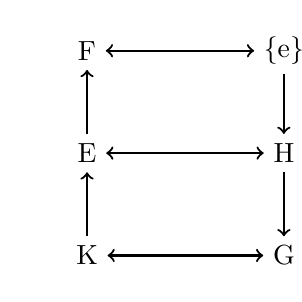
\begin{tikzpicture}
      \hspace{5mm}
      \node (f) {F};
      \node[below of=f, yshift=-3mm] (e) {E};
      \node[below of=e, yshift=-3mm] (k) {K};

      \draw[<-,thick] (f)--(e);
      \draw[<-,thick] (e)--(k);

      \node[right of=f, xshift=15mm] (i) {\{e\}};
      \node[below of=i, yshift=-3mm] (h) {H};
      \node[below of=h, yshift=-3mm] (g) {G};

      \draw[->, thick] (i)--(h);
      \draw[->, thick] (h)--(g);

      \draw[<->, thick] (f)--(i);
      \draw[<->, thick] (e)--(h);
      \draw[<->, thick] (k)--(g);
    \end{tikzpicture}
  \end{tcolorbox}
\end{minipage}

\vspace{5mm}
\begin{remark}
  The intermediate fields are getting larger as we go from top to bottom  as the fields are getting extended. But the subgroups are getting smaller.
\end{remark}

\vspace{7mm}
\section{Insights to the Fundamental Theorem}

\subsection{Nature of a Number}
The nature of a number depends upon the underlying field. As a field-automorphism of  \(\mathbb{Q}(\sqrt{2})\) that fixes \(\mathbb{Q}\) is \(\mathbb{Q}(-\sqrt{2})\) i.e \(\sqrt{2} \longmapsto -\sqrt{2}\). So,  any polynomial equation over \(\mathbb{Q}\) satisfied by the number \(\sqrt{2}\) is also satisfied by the number \(-\sqrt{2}\). You can fluidly pass between these two numbers and the equation with a rational coefficient will not know. \textit{Hence the two numbers \(\sqrt{2}\) and \(-\sqrt{2}\) are algebraically same over \(\mathbb{Q}\).}\\

But the map \(\sqrt{2} \longmapsto -\sqrt{2}\) is not an automorphism of the field \(\mathbb{Q}(\sqrt{2})\) fixing itself, i.e fixing \(\mathbb{Q}(\sqrt{2})\). The only automorphism of \(\mathbb{Q}(\sqrt{2})\) is the identity map. So, you cannot pass \(\sqrt{2}\) for \(-\sqrt{2}\) for every equation with coefficients in \(\mathbb{Q}(\sqrt{2})\). \textit{Hence the two numbers \(\sqrt{2}\) and \(-\sqrt{2}\) are not algebraically same over \(\mathbb{Q}(\sqrt{2})\).}
\vspace{7mm}

\begin{figure}[h]
  \centering
 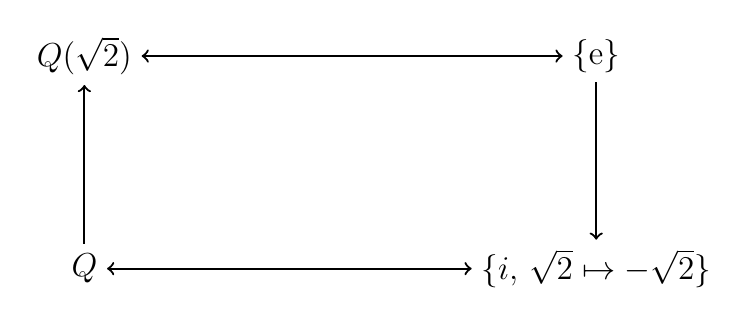
\begin{tikzpicture}
      \node (f) {\large \(\mathbb{Q}(\sqrt{2})\)};
      \node[below of=f, yshift=-17mm] (e) {\large \(\mathbb{Q}\)};


      \draw[<-,thick] (f)--(e);

      \node[right of=f, xshift=55mm] (i) {\large \{e\}};
      \node[below of=i, yshift=-17mm] (h) {\large \{\(i\), \(\sqrt{2} \mapsto -\sqrt{2}\)\}};


      \draw[->, thick] (i)--(h);


      \draw[<->, thick] (f)--(i);
      \draw[<->, thick] (e)--(h);
    \end{tikzpicture}
    \end{figure}
\clearpage

\subsection{Structure of a Field}
The structure of a field as an extension field over some field is mirrored in the structure of the ``group'' of  permutations of its elements that keeps the base field fixed. But these permutations are the symmetries of the field. \textit{So, the structure of field extension is equals to its own symmetry.}\\

The structure of a field is a \textbf{complicated} thing; specially if it is infinite. But the structure of a group is rather simple; especially if it is finite. So the Galois theory has fairly simplified the complicated thing in a very insightful and beautiful way.\\

Also Galois theory gives a new sights of study of fields which is ``study of fields via study of its automorphisms'' which are permutations of the field. That is\\[5mm]

\begin{figure}[h]
  \centering
  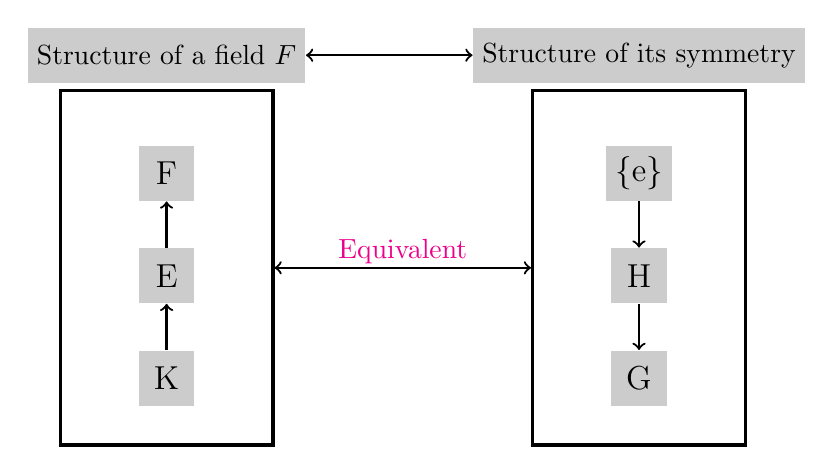
\begin{tikzpicture}

    \node[rectangle, very thick, draw,
    minimum height=4.5cm,
    minimum width=2.7cm] (rec) at (0,0) {};

    \node[rectangle, very thick, draw,
    minimum height=4.5cm,
    minimum width=2.7cm] (rec2) at (6,0) {};


    \node[minimum width=7mm,
      minimum height=7mm,
      fill=gray!40,
      ] (ss) at (0,2.7) {Structure of a field \(F\)};

      \node[minimum width=7mm,
      minimum height=7mm,
      fill=gray!40,
      ] (ss2) at (6,2.7) {Structure of its symmetry};

      \draw[<->, thick] (ss)--(ss2);
       \draw[<->, thick] (rec)--(rec2);

      \node[minimum width=7mm,
      minimum height=7mm,
      fill=gray!40] (f) at (0,1.2) {\large F};

      \node[minimum width=7mm,
      minimum height=7mm,
      fill=gray!40,
      below of=f, yshift=-3mm] (e) {\large E};

      \node[right of=e,
      xshift=20mm, yshift=3mm] (txt) {\textcolor{magenta}{Equivalent}};

      \node[minimum width=7mm,
      minimum height=7mm,
      fill=gray!40,
      below of=e, yshift=-3mm] (k) {\large K};

      \draw[<-,thick] (f)--(e);
      \draw[<-,thick] (e)--(k);

      \node[right of=f,
      xshift=5cm,
      minimum width=7mm,
      minimum height=7mm,
      fill=gray!40,
      ] (i) {\large \{e\}};

      \node[minimum width=7mm,
      minimum height=7mm,
      fill=gray!40,
      below of=i, yshift=-3mm] (h) {\large H};

      \node[
      minimum width=7mm,
      minimum height=7mm,
      fill=gray!40,
      below of=h, yshift=-3mm] (g) {\large G};

      \draw[->, thick] (i)--(h);
      \draw[->, thick] (h)--(g);
    \end{tikzpicture}
    \caption{\footnotesize Equivalency}
\end{figure}


\chapter{Structure of Galois Extension}
\section{Galois Group}
Let \(F\) be a field. The set \(Aut F\) of all field-automorphisms \(F \rightarrow F \) forms a group under the function composition.\\ \\
Let \(E\) and \(F\) be extension fields of a field \(K\).\\
If nonzero field-homomorphism \(\sigma : E \rightarrow F\) is a K-module homomorphism then\\
\(\sigma(k)=\sigma(k1_E)=k\sigma(1_E)=k1_F=k\).\hspace{7mm}
i.e, \(\sigma\) fixes \(K\) elementwise.\\ \\
Conversely, if field homomorphism \(\sigma : E \rightarrow F\) fixes K elementwise, then \(\sigma\) is a nonzero and for any \(u \in E\),\(\sigma(ku)=\sigma(k)\sigma(u)=k\sigma(u)\)
i.e \(\sigma\) is a K-module homomorphism.\\ \\
A field-automorphism \(\sigma \in Aut F\) which is also K-homomorphism is called K-automorphism. In other words, a field-automorphism \(\sigma \in Aut F\) that fixes K elementwise is called K-automorphism.\\ \\
The group of all K-automorphisms of \(F\) is called the Galois group of \(F\) over \(K\) and is denoted by \(Aut_K^F\).

\section{Galois extension}
Let \(E\) be an intermediate field and \(H\) be a subgroup of \(Aut_K^F\), then:
\begin{enumerate}
\item[i)] \(H' = \{v \in F | \sigma(v)=v, for all \sigma \in H \}\) is an intermediate field of the extension field \(F\) of \(K\).
\item[ii)] \(E' = \{\sigma \in Aut_K^F | \sigma(u)=u, for all u \in E\}=Aut_E^F\) is a subgroup of \(Aut_K^F\).
\end{enumerate}

The field \(H'\) is called the fixed field of subgroup H in F.

\subsection{Fixed Field}
We have,\\
\(H' \rightarrow fixed field \) \hspace{5mm} \(E' \rightarrow Aut_E^F\)\\
Let \(Aut_K^F = G\) then the field fixed by it is \(G'\).\\
It is not necessary that the field fixed by \(G\) is \(K\) i.e, \(G'=K\).\\

\textbf{Example}\\
For \(f(x)=x^3-2 \in Q[x]\). Let \(u \in F\) such that \(f(u)=0\) and \(F=Q[u]\).Then
\(G=Aut_Q^{Q(u)}={1}\) so, \(G'=F \neq K\).\\[2mm]

\textbf{Galois extension}\\
Let \(F\) be an extension field of \(K\) such that the fixed field of the Galois group \(Aut_K^F\) is \(K\) itself. Then \(F\) is said to be a Galois extension of \(K\) or to be Galois over \( K\).

\section{Fundamental Theorem of Galois Theory}

If \(F\) is a finite dimensional Galois extension of \(K\), then there is a one-to-one correspondence between the set of all intermediate fields of the extension and the set of subgroups of the Galois group \(Aut_K^F\) such that:
\begin{enumerate}
\item[i)] the relative dimension of two intermediate fields is equal to the relative index of the corresponding subgroups; in particular \(Aut_K^F\) has order \([F:K]\);
  \item[ii)] \(F\) is Galois over every intermediate field \(E\), but \(E\) is Galois over \(K\) if and only if the corresponding subgroup \(E'= Aut_E^F\) is normal in \(G=Aut_K^F\);in this case \(G/E'\) is isomorphic to the Galois group \(Aut_K^E\) of \(E\) over \(K\).
  \end{enumerate}

  We already have a correspondence between the intermediate fields and the subgroup of Galois group given by the fixed fields and the corresponding subgroups of the intermediate field \(E\), \(Aut_E^F\).
  i.e, to each intermediate field \(E\), there is a subgroup \(Aut_E^F\) and to each subgroup \(H\) there is a fixed field \(H'\).\\[2mm]
  But this correspondence is one-to-one if and only if \(E''=E\) and so on.

  \subsection{Closed Field and Subgroup}
  We have,
  \begin{enumerate}
  \item[i)] \(F'=1\) and \(K'=G\);
  \item[ii)] \(1'=F\);
    \end{enumerate}

    If \(F\) is Galois over \(K\) then by definition, \(G'=K\). Since \(K'=G\) we have \(K=K''\) if and only if \(F\) is Galois over \(K\).\\

    Let \(X\) be an intermediate field or subgroup of the Galois group. \(X\) will be called \textbf{closed} provided \(X=X''\).\\[3mm]

    \textbf{Theorem}. If \(F\) is an extension field of \(K\), then there is one-to-one correspondence between the closed intermediate fields of the extension and the closed subgroups of the Galois group, given by \(E \rightarrow E' =  Aut_E^F\).\\[3mm]

    \textbf{Lemma}. Let \(F\) be an extension field of \(K\), \(L\) and \(M\) intermediate fields with \(L \subset M\), and \(H\), \(J\) subgroups of Galois group \(Aut_K^F\) with \(H<J\).
    \begin{enumerate}
    \item[i)] If \(L\) is closed and \([M:L]\) finite, then \(M\) is closed and \([L':M']=[M:L]\);
    \item[ii)] if \(H\) is closed and \([J:H]\) finite, then \(J\) is closed and \([H':J']=[J:H]\);
      \item[iii)] if \(F\) is a finite dimensional Galois extension of \(K\), then all intermediate fields and all subgroups of the Galois group are closed and \(Aut_K^F\) has order \([F:K]\).
      \end{enumerate}

      \subsection{Stable Intermediate}
      \textbf{Lemma}. Let \(F\) be an extension field of K.
      \begin{enumerate}
      \item[i)] If E is a stable intermediate field of the extension, then \(E'=Aut_E^F\) is a normal subgroup of the Galois group \(Aut_K^F\);
        \item[ii)] if \(H\) is a normal subgroup of \(Aut_K^F\), then the fixed field \(H'\) of \(H\) is a stable intermediate field of the extension.
        \end{enumerate}

        \subsection{Proof of the Fundamental Theorem}
        From the above section there is one-to-one correspondence between closed intermediate fields of the extension and closed subgroups of the Galois group. But in this case all intermediate fields and all subgroups are closed. Thus follows Statement(i) of the theorem.\\[2mm]

        \(F\) is Galois over \(E\) since \(E\) is closed. \(E\) is finite dimensional over \(K\) since \(F\) is and hence algebraic over \(K\). Consequently, if \(E\) is Galois over \(K\), then \(E\) is stable.
        \(E'=Aut_E^F\) is normal in \(Aut_K^F\). Conversely if \(E'\) is normal in \(Aut_K^F\), then \(E''\) is stable intermediate field. But \(E=E''\) since all intermediate fields are closed and hence \(E\) is Galois over \(K\).\\[2mm]

        Suppose \(E\) is an intermediate field that is Galois over \(K\). Since \(E\) and \(E'\) are closed and \(G'=K\)(F is Galois over K), we have \(|G/E'|=[G:E']=[E''=G']=[E:K]\). So, \(G/E'=Aut_K^F/Aut_E^F\) is isomorphic to a subgroup of \(Aut_K^F\). But by first part of the theorem, \(|Aut_K^E|=[E:F]\)(since E is Galois over K). This implies \(G/E'=Aut_K^E\).



%%% Local Variables:
%%% mode: latex
%%% TeX-master: "n"
%%% End:




\part{Applications}
\chapter{Galois Group of a Polynomial}
\begin{definition}
  The Galois group of a polynomial \(f \in K[x]\) is the group \(Aut_K^F\), where \(F\) is a splitting field of \(f\) over \(K\).
  \end{definition}

  \begin{theorem}
  Let \(G\) be a Galois group of a polynomial \(f \in K[x]\).
\begin{enumerate}
\item[i)] \(G\) is isomorphic to a subgroup of some symmetric group \(S_n\)..
  \item[ii)] If \(f\) is separable of degree \(n\), the \(n\) divides \(|G|\) and \(G\) isomorphic to a transitive subgroup of \(S_n\).
  \end{enumerate}
\end{theorem}
Because the Galois group \(Aut_K^F\) is a group of automorphisms of F which is given by the permutations of the roots.
So, the Galois group of a polynomial is identified with the subgroup of \(S_n\).\\

\begin{corollary}
\begin{enumerate}
\item[i)] If the degree of \(f\) is \(2\) then its Galois group \(G \cong {\mathbb{Z}}_2\).
  \item[ii)] If the degree of \(f\) is \(3\) then its Galois group \(G\) is either \(S_3\) or \(A_3\).
  \end{enumerate}
\end{corollary}


\section{Galois Group of Cubic polynomials}
\begin{definition}
  Let \(K\) be a field with \(char K \neq 2\) and \(f \in K[x]\) a polynomial of degree \(n\) with \(n\) distinct roots \(u_1,u_2,...,u_n\) in some splitting field \(F\) of \(f\) over \(K\). Let \(\Delta = \prod\limits_{i<j}(u_i-u_j) = (u_1-u_2)(u_1-u_3)...(u_{n-1}-u_n) \in F\).\\
  The discriminant of \(f\) is the element \(D= {\Delta}^2\).
\end{definition}

\begin{theorem}
\begin{enumerate}
\item[i)] The discriminant \({\Delta}^2\) of \(f\) actually lies in \(K\).
  \item[ii)] For each \(\sigma \in Aut_K^F < S_n, \sigma\) is an even[resp. odd] if and only if \(\sigma(\Delta) = \Delta\)[resp. \(\sigma(\Delta) = - \Delta\)].
  \end{enumerate}
\end{theorem}
Since \({\Delta}^2 \in K\) and \(\Delta \in F\), and \(K(Delta)\) is a stable intermediate; in the Galois correspondence the subfield \(K(\Delta)\) corresponds to the subgroup \(G \cap A_n\). In particular, \(G\) consists of even permutations if and only if \(\Delta \in K\).

\begin{corollary}
  If \(f\) is a separable polynomial of degree \(3\), then the Galois group of \(f\) is \(A_3\) if and only if the discriminant of \(f\) is the square of an element of \(K\).
\end{corollary}

\begin{theorem}
  Let \(K\) be a field of \(char K \neq 2,3 \). If \(f(x)=x^3+bx^2+cx+d \in K[x]\) has three distinct roots in some splitting field, then the polynomial \(g(x)=f(x-b/3) \in K[x]\) has the form \(x^3+p^2+q\) and the discriminant of \(f\) is \(-4p^3-27q^2\) ~\cite{hunger}.
\end{theorem}

\section{Galois Group of Quartic polynomials}
\begin{definition}[Resolvant Cubic of a Quartic]
Let \(K, f, F, u_i, V,\) and \(G=Aut_K^F<S_4\) be as in the preceding paragraph and \(\alpha=u_1u_2+u_3u_4,\) \(\beta=u_1u_3+u_2u_4,\) \(\gamma=u_1u_4+u_2u_3\).
The polynomial \( (x- \alpha)(x- \beta)(x- \gamma) \) is called the resolvant cubic of \(f\). The resolvant cubic is actually a polynomial over \(K\).\\
\end{definition}
Now under the Galois correspondence the subfield \(K(\alpha, \beta, \gamma)\) corresponds to the normal subgroup \(V \cap G\) because \(K(\alpha,\beta,\gamma)\) is a splitting field of the resolvant cubic
whose Galois group is a subgroup of \(S_3\) and only normal subgroup of \(N\) of \(S_4\) with \(|N| \leq 6\) is \(V\).\\
Hence \(K(\alpha, \beta, \gamma)\) is Galois over \(K\) and \(Aut_K^{K(\alpha, \beta, \gamma)} = G/(G \cap V\).

\begin{remark} If \(K\) is a field and \(f = x^4+bx^3+cx^2+dx+e \in K[x]\), then the resolvant cubic of \(f\) is the polynomial \(x^3-cx^2+(bd-4e)x-b^2e+4ce-d^2 \in K[x]\).\\ \\
\end{remark}

\begin{theorem}
  Let \(K\) be a field and \(f \in K[x]\) a separable quartic with Galois Group \(G\). Let \(\alpha, \beta, \gamma\) be the roots of the resolvant cubic of \(f\) and let \(m= [K(\alpha, \beta, \gamma) : K]\) then,
\begin{enumerate}
\item[i)] \(m=6 \Longleftrightarrow G=S_4\);
\item[ii)] \(m=3 \Longleftrightarrow G=A_4\);
\item[iii)] \(m=1 \Longleftrightarrow G=V\);
\item[iv)] \(m=2 \Longleftrightarrow G=D_4\) or \(G={\mathbb{Z}}_4\); in this case \(G={\mathbb{Z}}_4\) if \(f\) is irreducible over \(K(\alpha, \beta, \gamma)\) and \(G={\mathbb{Z}}_4\) otherwise.
  \end{enumerate}
\end{theorem}
This is because we have \([K(\alpha,\beta,\gamma):K] = |G/G \cap V|\).

\section{Galois Group of some Polynomials}

\begin{example}
The polynomial is \(f(x)=x^4-2 \in \mathbb{Q}[x]\).\\
This polynomial is irreducible and so separable over \(\mathbb{Q}\). The resolvant cubic is \(x^3+8x = x(x+2i\sqrt{2})(x-2i\sqrt{2})\) and 
\(\mathbb{Q}(\alpha,\beta, \gamma)=\mathbb{Q}(i\sqrt{2})\) has dimension \(2\) over \(mathbb{Q}\).\\
\(x^4-2\) is irreducible over \(\mathbb{Q}(i\sqrt{2})\) because \(\sqrt[\leftroot{-3}\uproot{3}4]{2} \not\in \mathbb{Q}(i\sqrt{2})\).
Therefore the Galois group \(G \cong D_8\).
\end{example}








%%% Local Variables:
%%% mode: latex
%%% TeX-master: "n"
%%% End:


\chapter{Galois Fields}
Galois fields are the finite fields. They can be completely characterized in terms of splitting fields of some polynomials. It is found that the Galois group of an extension of a finite field by a finite field is cyclic. The Galois field with \(q\) elements is denoted by \(GF(q)\).

\begin{definition}[Prime Fields]
Let \(F\) be a field and let \(P\) be the intersection of all subfields of \(F\). Then \(P\) is a field with no proper subfields. This field \(P\) is called the Prime subfield of \(F\).
\end{definition}

\begin{enumerate}
\item If \(charF=p(prime)\), then \(P\cong {\mathbb{Z}}_p\).
\item If \(charF=0\), then \(P\cong \mathbb{Q}\).
\end{enumerate}

\begin{theorem}
A  finite field \(F\) has \(p^n\) number of elements where \(p \in \mathbb{Z}_+\) is a prime and it has \(p^n\) number of elements if and only if \(F\) is a splitting field of \(x^{p^n} - x\) over \(\mathbb{Z}_p\).\\
\end{theorem}

\begin{theorem}
  If \(F\) is a finite dimensional extension field of a finite field \(K\), then \(F\) is finite and is Galois over \(K\). The Galois group \(Aut_K^F\) is cyclic.
\end{theorem}

\section{Representation of Finite Fields}
Basically there are two types of representation of a finite field. These two representations are equivalent. 
\subsection{Integer representation}

\(GF(p^n)=\{0,1,...,p-1\} \cup \{p,p+1,...,p+p-1\} \cup ... \cup \{p^{n-1},p^{n-1}+1,...,p^{n-1}+p^{n-2}+...+p-1\}\).

\begin{example}
    \(GF(2)=\{0,1\}\)\\
    \(GF(2^3)=\{0,1\} \cup \{2,2+1\} \cup \{2^2,2^2+1,2^2+2,2^2+2+1\}=\{0,1,2,3,4,5,6,7\}\)
\end{example}

But the digits \(2,3,..,7\) of the field \(GF(2^3)\) do not lie on the field \(GF(2)\). If we look the field \(GF(2^3)\) as an extension field of \(GF(2)\) and write its elements using only the elements of the base field \(GF(2)\) then we have the following representations:
\vspace{3mm}

\begin{tabular}{|c|c|c|}
    \hline
    Digits & \ & Binary rep..\\
    \hline
    3 & \(2+1\) & 011 \\
    4 & \(2^2+2^1 \times 0 +2^0 \times 0\) & 100 \\
    5 & \(2^2+1\) & 110 \\
    \hline
\end{tabular}
\vspace{3mm}

This is actually \textbf{Binary representation} of the field \(GF(2^3)\)



\subsection{Polynomial representation}
For a field \(F\) and and an irreducible polynomial \(f(x) \in F[x]\) the quotient ring \(F[x]/(f(x))\) is field.\\
If \(F\) is a finite field consisting of \(p\) number of elements and \(f(x) \in F[x]\) is irreducible then \(F[x]/(f(x))\) is finite field. This field consists of all polynomials modulo \(f(x)\). If \(F=GF(2^3)\) then \(x^8+x^7+...+x+1 \in F[x]\) is irreducible in \(F[x]\). Since \(F\) has \(8\) elements which are modulo \(8\), \(F\) is represented by the factor ring \(F[x]/(f(x))\). \\


In the example above, the number \(5\) has the representation \(2^2+1\). This gives the polynomial representation \(x^2+1=(1,0,1)\)(coefficient of \(x^2\) is \(1\) of \(x\) is \(0\) and of constant is \(1\) ) Now the binary equivalent of \(5\) is \(101\).

\section{Operations in Galois Field}
Let the Galois field be \(GF(p^n)\). Since the elements of a Galois field can be represented as polynomials the operations are similar to polynomial operations. Let \(f(x)=a_0+a_1x+..+a_{n-1}x^{n-1}\) and \(g(x)=(b_0+b_1x+...+b_{n-1}x^{n-1}\).
\begin{enumerate}
  \item Addition \\
  \(f(x)+g(x)\;\;\;\; (modp)\) 
  \item Multiplicaiton \\
  \(f(x).g(x)\;\;\; (modp)\)
\end{enumerate}




\end{document}
%%% Local Variables:
%%% mode: latex
%%% TeX-master: t
%%% End:
